%
\documentclass[12pt]{article}

% The usual packages
\usepackage{fullpage}
\usepackage{breakcites}
\usepackage{setspace}
\usepackage{endnotes}
\usepackage{float}
\usepackage{amsmath}
\usepackage{amsfonts}
\usepackage{amssymb}
\usepackage{rotating}
\usepackage{dcolumn}
\usepackage{longtable}
\usepackage{microtype}
\usepackage{graphicx}
\usepackage{hyperref}
%\usepackage[usenames,dvipsnames]{color}
\usepackage{url}
\usepackage{natbib}
\usepackage{framed}
\usepackage{epigraph}
\usepackage{lipsum}
\usepackage[font=small,labelfont=sc]{caption}
\restylefloat{table}
\bibpunct{(}{)}{;}{a}{}{,}

% Set paragraph spacing the way I like
\parskip=0pt
\parindent=20pt

% Define mathematical results
\newtheorem{lemma}{Lemma}
\newtheorem{proposition}{Proposition}
\newtheorem{theorem}{Theorem}
\newtheorem{claim}{Claim}
\newenvironment{proof}[1][Proof]{\begin{trivlist}
\item[\hskip \labelsep {\bfseries #1}]}{\end{trivlist}}
\newenvironment{definition}[1][Definition]{\begin{trivlist}
\item[\hskip \labelsep {\bfseries #1}]}{\end{trivlist}}
\newenvironment{example}[1][Example]{\begin{trivlist}
\item[\hskip \labelsep {\bfseries #1}]}{\end{trivlist}}
\newenvironment{remark}[1][Remark]{\begin{trivlist}
\item[\hskip \labelsep {\bfseries #1}]}{\end{trivlist}}

% Set up fonts the way I like
\usepackage{tgpagella}
\usepackage[T1]{fontenc}
\usepackage[bitstream-charter]{mathdesign}

%% Set up lists the way I like
% Redefine the first level
\renewcommand{\theenumi}{\arabic{enumi}.}
\renewcommand{\labelenumi}{\theenumi}
% Redefine the second level
\renewcommand{\theenumii}{\alph{enumii}.}
\renewcommand{\labelenumii}{\theenumii}
% Redefine the third level
\renewcommand{\theenumiii}{\roman{enumiii}.}
\renewcommand{\labelenumiii}{\theenumiii}
% Redefine the fourth level
\renewcommand{\theenumiv}{\Alph{enumiv}.}
\renewcommand{\labelenumiv}{\theenumiv}
% Eliminate spacing around lists
\usepackage{enumitem}
\setlist{nolistsep}

% Create footnote command so that my name
% has an asterisk rather than a one.
\long\def\symbolfootnote[#1]#2{\begingroup%
\def\thefootnote{\fnsymbol{footnote}}\footnote[#1]{#2}\endgroup}

% Create the colors I want
\usepackage{color}
\definecolor{darkred}{RGB}{100,0,0}

\hypersetup{
 pdftitle={Meaningful Inferences}, % title
 pdfauthor={Kelly McCaskey and Carlisle Rainey}, % author
 pdfkeywords={hypothesis testing} {confidence intervals} {substantive significance}
 pdfnewwindow=true, % links in new window
 colorlinks=true, % false: boxed links; true: colored links
 linkcolor=darkred, % color of internal links
 citecolor=darkred, % color of links to bibliography
 filecolor=darkred, % color of file links
 urlcolor=darkred % color of external links
}

% enable comments in pdf
\newcommand{\kelly}[1]{\textcolor{blue}{#1}}
\newcommand{\carlisle}[1]{\textcolor{magenta}{#1}}


\begin{document}

\begin{center}
{\LARGE Meaningful Inferences}\\\vspace{2mm}
{\large The Importance of Explicit Statistical Arguments for Substantive Significance\symbolfootnote[1]{We thank [many people]. Thanks to Lisa Hultman, Jacob Kathman, and Megan Shannon and Cindy D. Kam and Elizabeth J. Zechmeister for making their data available to us. The analyses presented here were conducted with \texttt{R} 3.1.0 and Stata 13. All data and computer code necessary for replication are available at \href{https://github.com/carlislerainey/meaningful-inferences}{github.com/carlislerainey/meaningful-inferences}.}}\\\vspace{2mm}


\vspace{10mm}

Kelly McCaskey\symbolfootnote[2]{Kelly McCaskey is a Ph.D. student in the Department of Political Science, University at Buffalo, SUNY, 520 Park Hall, Buffalo, NY 14260 (\href{mailto:kellymcc@buffalo.edu}{kellymcc@buffalo.edu}).}

\vspace{3mm}

Carlisle Rainey\symbolfootnote[3]{Carlisle Rainey is Assistant Professor of Political Science, University at Buffalo, SUNY, 520 Park Hall, Buffalo, NY 14260 (\href{mailto:rcrainey@buffalo.edu}{rcrainey@buffalo.edu}).}
\end{center}

\vspace{10mm}

% Abstract
{\centerline{\textbf{Abstract}}}
\begin{quote}\noindent
Research in political science is gradually moving away from an exclusive focus on statistical significance testing and toward an emphasis on effect magnitude. We argue that the current practice of ``magnitude-and-significance,'' in which researchers interpret only the magnitude of a statistically significant estimate is only a small improvement over the much maligned ``sign-and-significance'' approach, in which researcher focus only on the statistical significance of an estimate. We argue that instead of interpreting the magnitude of a statistically significant effect, researchers should explicitly account for uncertainty when making judgments about substantive importance of statistical results. This requires the researcher to precisely define the effects that are and are not substantively meaningful and show that those effects are unlikely to generate the observed data. Using the effect of U.N. troops on civilian casualties during civil war and the effect of yard signs on candidate support, we show that our approach might strengthen or weaken claims of substantive significance. 
 \end{quote}

% Add quote to first page
\epigraph{Far better an approximate answer to the \textit{right} question, which is often vague, than an exact answer to the \textit{wrong} question, which can always be made precise.}{\citet[pp. 13-14]{Tukey1962}}

% Remove page number from first page
\thispagestyle{empty}

% Start main text
\newpage
\doublespace

\section*{Introduction}

% This paragraph gives an overview of the paper. However, I'm not sure that it is needed, since it largely duplicates the abstract. Instead, perhaps we should lead with examples of claims about substantive significance?
Recent work in political science encourages researchers to move beyond statistical significance and focus on the \emph{substantive importance} of the \emph{magnitude} of the effect (e.g., \citealt{KingTomzWittenberg2000}; \citealt{HanmerKalkan2013}; and\citealt{EsareyDanneman2014}). The current practice argues for substantive importance by interpreting the magnitude of statistically significant estimates. If the estimate is substantively large, then the researcher concludes the effect is ``substantively and statistically significant.'' However, we do not find this approach compelling. Indeed, we argue that focusing on the magnitude of the only estimated effect retains many of the flaws associated with focusing \emph{only} on statistical significance. Instead, researchers should take the uncertainty of the estimates into account when arguing for substantive significance. Following \cite{Gross2014} and \cite{Rainey2014}, we suggest that researchers carefully define the set of effects that are and are not substantively meaningful and then explicitly test the hypothesis that the estimated effect is substantively meaningful.

% There are three questions that political scientists care about.
We contend that the best empirical political science concerns itself with three questions about the causal effects of interest. 

\begin{enumerate}
\item What is the direction of the effect?
\item How large is the effect?
\item Is the effect substantively important?
\end{enumerate}

% Two of them are usually addressed
Each of these questions require increasing levels of analysis and substantive interpretation and each receives decreasing levels of attention in political science research. Virtually every research article in empirical science makes an argument about the direction of the effect using a null hypothesis significance test. Almost all of these articles report some measure of effect size, even if it is just in the form of a table of regression coefficients. 

% The third is usually not.
However, judgments about the importance of the effect are often missing. To get a sense of how often researchers address substantive importance (i.e., Are the effects large enough to care about?), we reviewed all articles published in the \textit{American Political Science Review} and the \textit{American Journal of Political Science} from 2011 to 2013. Of the 316 total articles, 73\% were empirical analyses. Of this 73\%, only about half make a judgment about the substantive importance of the estimated effect. Furthermore, of the articles that discuss the substantive importance of their results, only 17\% make an explicit argument that the estimates are substantively large.

% Overview of the paper
We begin by elaborating on the questions that political scientists typically ask about effects and explain the typical approaches to answering these questions. We then overview the much maligned sign-and-significance approach to arguing for meaningful effects and the current best practice of magnitude-and-significance. We then explain why the magnitude-and-significance approach is only a small improvement over the sign-and-significance approach. As an alternative, we suggest that researchers carefully define the set of effects and are and are not substantively meaningful and then formally test the hypothesis that the estimated effect is substantively meaningful. 

\section*{What We Want To Know}

% What we mean by "an effect."
Most empirical research in political science focuses on estimating the effect $\Delta$ of an explanatory variable $x$ on the expected value of an outcome of interest $y$. Formally, we might suppose that $E(y | x) = f(x)$ and define the ``effect'' or ``quantity of interest'' $\Delta$ as the difference between the average outcomes when $x$ takes on a substantively meaningful high value and low value, so that $\Delta = E(y | x = x_{hi}) - E(y | x = x_{lo}) = f(x_{hi}) - f(x_{lo})$. Importantly, empirical work usually focuses on answering three fundamental questions about the effect $\Delta$ of $x$ on $E(y|x)$. 

\begin{enumerate}
\item What is the direction of the effect?
\item How large is the effect?
\item Is the effect substantively important?
\end{enumerate}

%For example, consider the effects of U.N. troops on civilian casualties during a civil war \citep{HultmanKathmanShannon2013}. The first question concerns the direction of the effect. It could be that the troops have the intended effect and reduce casualties. However, the troops might also have the unintended consequences of antagonizes the parties to the conflict and increasing civilian casualties. 

%Once we establish the direction of the effect, we next want to know how large the effect is. Supposing a benefit, on average, does a commitment of 5,000 troops save 5, 50, or 500 civilians? 

%Once we establish the magnitude of an effect, we want to make a substantive judgement about the importance of that effect. If committing the troops saves only 5 lives, then researchers would probably consider that a substantively negligible effect since organizations would consider alternative strategies. However, if committing the troops saves 500 lives, then researchers would probably recognize that as a meaningful benefit and argue that the presence of U.N. troops leads to a substantively meaningful decrease in civilian casualties.

\subsection*{Direction}

% Orient the reader to the direction question
The first question that question that empirical research usually attempts to answer is the direction of the effect. Is the effect positive or negative?\footnote{Some research argues theoretically and empirically for ``no effect'' or ``a negligible effect'' (e.g., \citealt{KamPalmer2008}, see \citealt{Rainey2014}), but most hypotheses posit the direction of an effect.} 

% Provide the details of the direction question
Suppose, for clarity, that the researcher offers a directional research hypothesis, suggesting that an effect of interest $\Delta$ is positive. Formally, we might denote this hypothesis as $H_r: \Delta > 0$. Then the researcher compares this research hypothesis to a null hypothesis that suggests that the research hypothesis is false, or equivalently, that the effect lies outside the region suggested by the research hypothesis. Formally, we might write this as $H_0: \Delta \leq 0$. To assess the evidence against the null hypothesis, the researcher usually calculates a $p$-value, which is the probability of obtaining (hypothetical) data at least as extreme as the observed data if the null hypothesis were true.\footnote{This is always the case in our sample.} If this $p$-value is sufficiently small (by convention, less than 0.05), then the researcher rejects the null hypothesis in favor of the research hypothesis. In our example, the researcher would reject negative effects and conclude that the effect is positive. However, if the $p$-value is not sufficiently small, then the researcher declares that the data do not offer compelling evidence against the null and notes that the direction of the effect remains uncertain.\footnote{However, some research takes a $p$-value greater than 0.05 as evidence \textit{in favor of} the null hypothesis \citep{Rainey2014}. We prefer to interpret a lack of statistical significance as ambiguous evidence from which the researcher can make no claim (i.e., the effect might be negative or positive).}

%\cite{WilsonPiazza2013} provide an example of this ``sign-and-significance'' approach. They hypothesize that both democratic and military regimes are more likely to experience terrorism than single-party regimes. They use a reference regime to compare for each model and discuss the implications in terms of the sign and significance of the coefficient. In particular, they find that ``party-based autocracies are significantly more likely to have no terrorism in a given year,'' and that ``this relationship is confirmed true below a 0.01 probability of error'' (p. 949). %They also find, due to a $p$-value greater than 0.1, that the number of expected terrorist attacks in military regimes as compared to democracies are not statistically distinguishable. Though the authors do not, this may be an instance where it is possible to interpret this lack of statistical significance as ambiguous evidence to which we can make no claim rather than group the two regimes together. 

% Three things to note about arguments for direction.
There are features of arguments for direction to make note of. First, this style of argumentation is ubiquitous in political science. It is extremely rare to find empirical research in political science that does not perform a hypothesis test of some sort. Each empirical study published in the \textit{APSR} and \textit{AJPS} from 2011 to 3013 performs some type of hypothesis test. Second, this approach is compelling not because it argues that the observed data are consistent with the researcher's claim, but because the data are inconsistent with other claims. Third, this argument for the direction of the effect explicitly accounts for the uncertainty of the estimated effect. If the uncertainty is large relative to the magnitude of the estimate then the researcher cannot (and usually does not) make confident claims about the direction of the effect of interest. However, if the uncertainty is small relative to the size of the estimated effect, then the researcher can draw confident conclusions about the direction of the effect. 

\subsection*{Magnitude}

% Orient the reader toward the magnitude question
Yet recent methodological work emphasizes that empirical work should go beyond estimating the direction of the effect (\citealt{KingTomzWittenberg2000}; \citealt{HanmerKalkan2013}; \citealt{Gross2014}). In addition to the direction of an effect, the size of the effect matters as well. 

%% Provide the details of the magnitude question
However, computing an interpretable measure of effect magnitude is not always straightforward. Only some statistical models have naturally interpretable parameters. For example, a simple difference-in-means or normal-linear model have directly interpretable coefficients as long as the scales of the variables are reasonable and the model does not include non-linear or product terms. Outside of these atypical situations, however, the researcher must do additional work to estimate a substantively meaningful quantity of interest.

% King quote on importance of magnitude
In discussing how scholars might interpret a model of the effects of education on income, \citet[p. 348]{KingTomzWittenberg2000} write:

\begin{quote}
Bad interpretations are substantively ambiguous and filled with methodological jargon: ``the coefficient on education was statistically significant at the 0.05 level.'' Descriptions like this are very common in social science, but students, public officials, and scholars should not need to understand phrases like ``coefficient,'' ``statistically significant,'' and ``the 0.05 level'' to learn from the research. Moreover, even statistically savvy readers should complain that the sentences does not convey the key quantity of interest: how much higher the starting salary would be if the student attended college for an extra year.
\end{quote}

% However, the idea that magnitude is important has been around a while
The emphasis on effect magnitude is not a new idea. Commenting on the consequences of Fisher's null hypothesis significance test, \citet[p. 32]{Yates1951} writes: ``[I]t has caused scientific workers to pay undue attention to the results of the tests of significance they perform on their data, particularly data derived from experiments, and too little to the estimates of the magnitude of the effects they are investigating.'' Yates continues: 

\begin{quote}
Tests of significance are preliminary or ancillary. The emphasis on tests of significance, and the consideration of the results of each experiment in isolation, have had the unfortunate consequence that scientific works have regarded the execution of a test of significance on an experiment as the ultimate objective. Results are significant or not significant and that is the end of it (p. 33).
\end{quote}

% Substantively interpretable measures of magnitude are easy.
Fortunately, recent conceptual work (\citealt{KingTomzWittenberg2000}; \citealt{BerryDeMerittEsarey2010}; and \citealt{HanmerKalkan2013}) and software development (\citealt{TomzWittenbergKing2003}; and \citealt{ImaiKingLau2007}) empowers political scientists to move beyond a simple ``sign-and-significance'' approach and also present substantively meaningful measures of effect magnitude.

\subsection*{Importance}

% Orient the reader to the question of importance
But ultimately, researchers want to move beyond the simple presentation of effect magnitude and make a judgment about the meaningfulness of the effects. Is the effect large or small? Is it substantively important? Is it relevant for policy? Is it scientifically important? Is it large enough to matter? \citet[p. 264]{HanmerKalkan2013} write: ``[W]e take it as given that understanding whether the relationship is substantively significant, rather than just statistically significant, is the ultimate goal, as it is a necessary part of vaulting one's theory.''

% one example of a claim of importance
For example, \citet[p. 711]{KingZeng2001} claim that, ``if a collection of 300,000 dyads shows a 0.001 increase in the probability of war, the finding is catastrophically \emph{important because} it represents about three hundred additional wars and a massive loss of human life'' (emphasis ours).

%For example, \cite{Kinne2013} presents effects that he deems as substantively large enough to be important. He hypothesizes that there are three discernible ways that states network and form bilateral agreements and determines whether or not these are both statistically and substantively significant through his empirical analysis. Kinne interprets the substantive meaning of his results as states being ``73\% more likely to propose an agreement" or cooperate when there is a third party involved than any other combination of states and bilateral agreements (p. 778). By determining which effects are substantively meaningful, he is able to make the claim that his research makes a substantial contribution to the literature on international cooperation. His analysis ``puts endogenous influences in the spotlight, treating them not as methodological nuisances but as phenomena of substantive importance," and finds that typical much-cited cooperation influences ``diminish in substantive significance once network influences enter the equation" (p. 781). 

% and another example
%\citet[p. 317]{HetheringtonSuhay2011} note that 

\begin{quote}
When we fixed trust at its minimum, the predicted probability that our typical respondent thought Iraq was worth the cost was only 0.33; we would classify him as not believing Iraq was worth the cost. If we increase political trust to its maximum, however, the predicted probability more than doubles to .72, a 39 percentage point increase. This is substantively \emph{important because}, with trust at its maximum, our typical respondent believes Iraq was worth the cost.
\end{quote}


\section*{Current Practices in Reasoning About Effect Importance}

% Brief summary of the sign-and-significance approach
Two current practices dominate the way that researchers make statistical arguments for substantive significance. We argue that both of these approaches are flawed and we offer a third, improved method. First, researchers might deem any statistically significant result as an important one. We refer to this as the ``sign-and-significance'' approach in which researchers simply note the sign of an effect and claim it is statistically significant. This approach  interprets the $p$-value as a measure of magnitude or importance.

% Brief summary of the magnitude-and-significance approach
The second practice, which is more common in political science, is to interpret the magnitude without explicitly accounting for the uncertainty of the estimate. We refer to this as the ``magnitude-and-significance'' approach in which researchers first check that an effect is statistically significant and then interprets the magnitude of the estimate. While the magnitude-and-significance approach is no doubt and improvement on the sign-and-significance approach, it retains many of its flaws.

% Brief summary of the explicit-test approach
As an alternative, we suggest the explicit-test approach. To explicitly test a hypothesis of a meaningful effect, researchers simply use their substantive judgement to partition the set of possible effects into meaningful effects and trivial effects. They then conduct a formal hypothesis test that the true effect lies about the smallest substantively meaningful effect. This approach address the flaws of both the sign-and-significance and magnitude and significance approaches.

\subsection*{Sign-and-Significance}

% Overview of the SS approach
Using the sign-and-significance approach, researchers declare an effect important if and only if the effect is statistically significant. That is, researchers simply test whether the effect is greater than (or less than) zero. If the they reject the null (e.g., $p < 0.05$), then they declare the effect to be substantively meaningful.

% The problems with the SS approach
The much maligned (e.g., \citealt{Cohen1990}, \citealt{Gill1999}, \citealt{HillJones2014}, and \citealt{Gross2014}) sign-and-significance approach emphasizes $p$-values, but a minuscule $p$-value does not imply a large or important effect. The $p$-value depends on both the sample size and the effect size. It is true that the $p$-value gets smaller as the effect size under investigation increases. However, the $p$-value also decreases the sample size, which is unrelated to the effect size, increases. While it is common to describe estimates as ``highly significant'' or ``very significant,'' this implies (or tempts readers to conclude) that an effect is large or important. ``Very significant'' (e.g., $p < 0.001$) might simply mean that the researcher has a large sample. Even if the researcher finds statistically significant results with a small sample, the small $p$-value only indicates that the effect size is large relative to the uncertainty. It says nothing about the size of the estimate relative to some standard of substantive importance. With a very small $p$-value (e.g., $p < 0.001$), substantive experts might judge the effect to be large, moderate, small, or even negligible. Experts might call some of these effect important, somewhat important, slightly important, or not at all important. The $p$-value is indirectly related to substantive significance at best.

\subsection*{Magnitude-and-Significance}

% Overview of the MS approach
The standard scientific practice in political science is to take the magnitude-and-significance approach. 

\begin{enumerate}
\item Computes substantively interpretable estimate of the effect of interest, such as a first difference.
\item Test whether these estimates are statistically significant.
\item If so, make a judgement about whether the magnitude is substantively important.
\end{enumerate}

% Example 1
For example, \cite{TomzWeeks2013} discuss the results of their experiment on attitudes about conflict.

\begin{quote}
Citizens in both countries were much less willing to attack another democracy than to attack an otherwise equivalent autocracy. Approximately 34.2\% of respondents in the U.K. supported a military strike when the country was not a democracy versus 20.9\% when the country was a democracy. Thus, democracy reduced support for a military strike by more than 13 percentage points, with a 95\% confidence interval of 19.6 to 6.9. The baseline level of militarism was much higher in the United States, where at least half the respondents wanted to strike an autocracy. Nonetheless, democracy exerted a similarly large effect in the United States: The between-subjects and within-subject estimates concurred that democracy reduced enthusiasm for a military strike by about 11.5 percentage points. In both countries, democracy produced \emph{substantively large and statistically significant} effects on preferences (p. 854-855, emphasis ours).
\end{quote}

% Example 2
\cite{GerberHopkins2011} discuss their regression model.

\begin{quote}
The first model indicates that all else equal, a city where the Democrat just wins the mayoralty should expect its spending on police to drop by 2.3 percentage points three fiscal years later. This result is \emph{statistically significant}, with a 95\% confidence interval that runs from 0.5 percentage points to 4.0 percentage points. It is \emph{substantively large as well}, as it reflects a spending shift of 1.2 standard deviations in terms of the dependent variable (p. 333, emphasis ours).
\end{quote}

% Example 3
\cite{AnsolabehereJones2010} discuss their coefficients of their regression model.

\begin{quote}
The regression results in [their] Table 3 show that a Representative's actual roll-call votes strongly predict respondents' beliefs about the Representative's votes. The coefficients for both 2005 and 2006 are \emph{substantively large} (approximately 0.3) \emph{and statistically significant} (p. 588, emphasis ours). 
\end{quote}

% Problems with the MS approach
The magnitude-and-significance approach has three unfortunate consequences. It tempts researchers to...

\begin{enumerate}
\item treat all statistically significant and substantively large estimates similarly, drawing no distinction between large, imprecise estimates and large, precise estimates.
\item treat ``barely significant,'' large estimates and ``almost significant,'' large estimates quite differently, drawing a strong distinction between two similar estimates with similar uncertainty.
\item treat all results that are not statistically significant similarly, drawing no distinction between large, imprecise estimates and small, precise estimates (see Rainey 2014).
\end{enumerate}

% Introduce the example cis figure
Consider, for example the hypothetical studies presented in Figure \ref{fig:example-cis}. If we are interested in substantive significance and consider 0.25 as the minimal substantively meaningful effect, then only one study, Study A, seems to offer evidence for a substantively meaningful effect. After that, Studies B and C offer ambiguous evidence for a meaningful effect and Studies D and E offer evidence \emph{against} a meaningful effect.

% It treats studies A and B the same
Although only Study A offers compelling evidence for a meaningful effect, the magnitude-and-significance approach suggests that Studies A and B offer similar evidence for a substantively meaningful effect as well, since both are ``statistically significant and substantively large.''  Yet these studies do not offer similar evidence for a meaningful effect. Study A is only consistent with a meaningful effect. And while a large, meaningful effect is certainly plausible based on Study B, it fails to rule out small, negligible effects.

% It treats B and C differently
Instead, the amount of evidence for a meaningful effect offered by Study B is similar to that offered by Study C--both studies are consistent with both large and small effects. Yet the magnitude-and-significance approach treats these studies \emph{differently}. The magnitude-and-significance approach concludes that the effect is ``positive, significant, and substantively meaningful'' from Study B and ``not statistically significant'' from Study C.

% It treats C and E the same
The magnitude-and-significance approach also treats Studies C and E similarly because both estimates are ``not statistically significant.'' However, Study C is consistent with both large, meaningful effect and small, negligible effects. Study E on the other hand, is only consistent with small, negligible effects.

% The MS approach has many of the same problems as the SS approach.
In fact, the only improvement of the magnitude-and-significance over the much maligned sign-and-significance approach is that the current practice managed to distinguish between Study A and Study D. Other than that, both of these approaches treat Study A and B similarly, Studies B and C differently, and Studies C and E similarly. From our perspective, these are all inferential errors. Table \ref{tab:example-cis} shows the interpretation from each approach compared with an ``intuitive approach'' based on the confidence intervals. Especially notice the similar errors made by the dismissed sign-and-significance approach and the current practice of magnitude-and-significance.

\begin{figure}[h]
\begin{center}
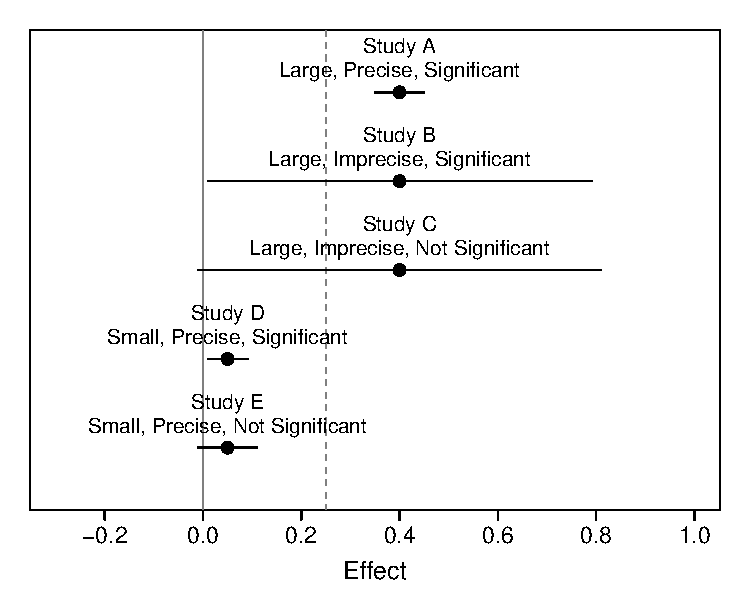
\includegraphics[scale = .8]{figs/example-cis.pdf}
\caption{This figure provides several hypothetical studies to illustrate several points about arguments for substantive significance. Notice that Study A offers compelling evidence for a meaningful effect, Studies B and C are consistent with both small and large effects, and Studies D and E offer evidence \emph{against} meaningful effects. However, the current practice in political science of magnitude and significance treats Studies A and B similarly, Studies B and C \emph{differently}, and Studies C and E similarly. Table \ref{tab:example-cis} for the interpretations from both the sign-and-significance and magnitude-and-significance approaches with the intuitive meaning.}\label{fig:example-cis}
\end{center}
\end{figure}

\renewcommand{\arraystretch}{1.5}
\begin{table}
\begin{center}
\begin{scriptsize}
\begin{tabular}{|>{\centering\arraybackslash}m{.5in}>{\centering\arraybackslash}m{1.75in}>{\centering\arraybackslash}m{1.75in}>{\centering\arraybackslash}
m{1.75in}|}
\hline
Study & Sign-and-Significance Method & Magnitude-and-Significance & Intuitive Interpretation\\ 
\hline
Study A & ``positive and significant'' & ``positive, significant, and substantively large'' & ``We have strong evidence for a large, substantively meaningful effect.''\\
Study B & ``positive and significant'' & ``positive, significant, and substantively large'' & ``We have only weak evidence for a large, substantively meaningful effect, because the data are also consistent with negligible effects near zero.''\\
Study C & ``not statistically significant'' & ``not statistically significant'' & ``We have only weak evidence for a large, substantively meaningful effect, because the data are also consistent with negligible effects near zero.''\\
Study D & ``positive and significant'' & ``positive and significant, but substantively small' & ``We have strong evidence against a substantively meaningful effect.''\\
Study E & ``not statistically significant'' & ``not statistically significant'' & ``We have strong evidence against a substantively meaningful effect.''\\
\hline
\end{tabular}\caption{This table compares the interpretations of the results in Figure \ref{fig:example-cis} using the sign-and-significance and the magnitude-and-significance approaches to the intuitive meaning of the confidence intervals. Notice that the much maligned sign-and-significance approach and the magnitude-and-significant approach only differ in their interpretations of Studies D and E. Both approaches deviate substantially from the intuitive interpretation based on the confidence intervals.}\label{tab:example-cis}
\end{scriptsize}
\end{center}
\end{table}

% We need to be consistent with the standard of evidence
It is important to apply similar standards of evidence to arguments for positive (or negative) and arguments for \emph{meaningfully} positive (or negative) effects. The usual logic of hypothesis testing requires that the researcher only declare that an effect is positive if and only if the evidence overwhelmingly points toward a positive (or negative). Similarly, researchers should not declare a positive estimate substantively meaningful simply because it is inconsistent with with negative effects and the point estimate lies above some threshold. A consistent standard of evidence requires that researchers declare an effect meaningful if and only if it is inconsistent with negligible effects.

\section*{A Compelling Argument for a Meaningful Effect}

% Overview of how we'll go about the problem
Researchers can make much more compelling and transparent arguments for meaningful effects by explicitly testing the claims we are making. For example, if  a researcher claims that an effect is positive and substantively meaningful, then the research hypothesis is not $H_r: \Delta > 0$. Instead, it's $H_r: \Delta > m$, where $m$ represents the researchers judgment about the smallest substantively interesting effect (or the largest substantively negligible effect). There is no need to jettison the entire hypothesis testing framework. In fact, the problems identified above can be addressed and the usual hypothesis testing framework can be kept intact if researchers are simply willing to apply their substantive judgment about which effects are and are not meaningful to their hypotheses rather than the estimated magnitude (see \citealt{Rainey2014} and \citealt{Gross2014}). 

% The specific steps
We propose the following procedure:

\begin{enumerate}
\item Hypothesize that the effect is positive and substantively meaningful (or negative and substantively meaningful).
\item Make a substantive judgment about the smallest substantively meaningful effect. That is, choose an $m$ such that $m$ represents the smallest substantively meaningful effect.
\item Test the research hypothesis $H_r: \Delta > m$ using a conventional hypothesis testing approach.
\end{enumerate}

\subsection*{Stating a Research Hypothesis of a Meaningful Effect}

% Overview
The first step is easy, but important. In order to make a compelling argument for a meaningful effect, researchers must clearly state their claims. Rather than simply hypothesizing that an effect is positive or negative, researcher must make their claim that a variable has a meaningful effect from the outset. 

% Example
For example, \cite{LevenduskyHorowitz2012} hypothesize that ``bipartisan support in Congress for the president's policy should decrease audience costs.'' Notice that this hypothesizes a direction, but not a magnitude of the effect. Yet in discussing this hypothesis, Levendusky and Horowitz write: 

\begin{quote}
This type of unexpected (disconfirming) cue has an \emph{especially large effect} on voters' decision-making processes. In effect, it sends voters a strong signal that this is not a partisan decision, but rather a decision about what is best for the nation. Further, the fact that even the president's rivals supported his decision suggests to voters that the president did make the right call, which should lead all voters (regardless of partisan affiliation) to punish the president less harshly, thereby minimizing audience costs (p. 326, emphasis ours).
\end{quote}

\noindent Thus, Levendusky and Horowitz carefully theorize about the magnitude of the effect, but ultimately offer a directional hypothesis. They could improve the test of their theory by building the implication about the size of the effect directly into their hypothesis, predicting that ``bipartisan support in Congress for the president's policy should \emph{substantially} decrease audience costs.'' We have simply added ``substantially'' to their hypothesis. This provides a strong indication to readers (and the researcher) that the theory implies the effect should be large and the researcher will provide a strong argument for a large negative effect, as opposed to simply a negative effect. 

\subsection*{Choosing $m$}

% Overview
In order to make a compelling argument that an effect is substantively meaningful, the researcher must carefully define exactly which effects are and are not substantively meaningful. To do this, researchers simply choose an $m$ such that effects smaller than $m$ are considered substantively negligible and effects larger than $m$ are consider substantively meaningful. This $m$ that partitions the possible effects into those that are substantively meaningful and those that are substantively negligible.

% We must insist on subjectivity.
As Rainey notes, political scientists should not insist on hard and fast rules for judging the effects that are and are not substantively meaningful.\footnote{We should note, though, that such rules of thumb have been presented, see \cite{Glass1976} and \cite{Cohen1992}, but these rules are usually proposed with caution.} Instead, we must insist that substantive scholars making substantive claims about politics also make substantive judgments about the importance of their effects. \citet[pp. 82-83]{Thompson2001} notes for example, that ``if people interpreted effect sizes with the same rigidity that $\alpha = 0.05$ has been used in statistical testing, we would merely be being stupid in another metric.'' \cite{Kirk1996} notes that this judgment is ``influenced by a variety of factors, including the researcher's value system, societal concerns, assessment of costs and benefits, and so on." Despite this element of subjectivity, \cite{Thompson2002} writes: 

\begin{quote}
The existence of effect size benchmarks should not justify abrogating the responsibility for arguing for effect import in the specific context of a given study. It is not necessary to have universal benchmarks regarding what effect sizes may be deemed noteworthy. The reader with a value system widely different than that of an author might reasonably disagree with the author about whether the effect size is noteworthy and then simply ignore the study.
\end{quote}

% Choosing m is subjective, but hypothesis tests are opaque 
Formal hypothesis tests and judgments about substantive importance are qualitatively different decisions and have different strengths and weaknesses. Estimation and hypothesis tests are relatively automatic and ``objective,'' but not transparent. Researchers do not fit one model and report the single $p$-value. Instead they fit many models and report the one that ``makes most sense'' in light of their approach, theoretical model, normative concerns, and the results of the model. (\citealt{GerberMalhotra2008}; \citealt{SimmonsNelsonSimonsohn2011}; \citealt{Francis2013}; \citealt{SimmonsNelsonSimonsohn2014}; and \citealt{EsareyWu2014}; see also \citealt{GelmanLoken2014}). Substantive judgments about effect sizes, however, require a large initial investment of careful thought and this judgment demands subjectivity. However, this subjective judgment is transparent. Readers are free to reject the author's judgment and substitute their own. Further, ``automatic'' and ``objective'' procedures are not always (or perhaps usually) desirable.  Indeed, \cite{Kirk1996} writes:

\begin{quote}
Researchers have an obligation to make this kind of judgment. No one is in a better position than the researcher who collected and analyzed the data to decide whether or not the results are trivial. It is a curious anomaly that researchers are trusted to make a variety of complex decisions in the design and execution of an experiment, hut in the name of objectivity, they are not expected or even encouraged to decide whether data are practically significant (p. 755).
\end{quote}

\noindent Substantive scholars making substantive points about politics must not be prohibited from making substantive judgments. Instead, they must be \emph{encouraged} to do so \citep{Achen1982}.

\section*{Testing a Hypothesis of a Meaningful Effect}

% Overview
Once the researcher has clearly identified that set of effects that he considers substantively meaningful, the testing problem is straightforward. For an effect of interest $\Delta$, the a researcher positing a ``substantively meaningful, positive effect'' must simply test her research hypothesis $H_r: \Delta > m$ against the null hypothesis $H_0: \Delta \leq m$. For a researcher positing a ``substantively meaningful, negative effect'' must simply test her research hypothesis $H_r: \Delta < -m$ against the null hypothesis $H_0: \Delta \geq -m$.\footnote{Though rarely used in practice, this the way hypothesis testing is introduced in in introductory textbooks (e.g., \citealt{WonnacottWonnacott1990}.}

% Example of the t-statistic
The case of $t$-statistics illustrates the parallel between testing for a meaningful positive effect and simply testing for a positive effect. If a researcher simply wishes to argue that an effect is positive (though perhaps substantively irrelevant), the $t$-statistic is given by $t = \dfrac{\Delta}{\sqrt{\widehat{Var}(\Delta)}}$. If a researcher wishes to argue that an effect is positive and substantively meaningful, then the required $t$-statistic is given by $t = \dfrac{\Delta - m}{\sqrt{\widehat{Var}(\Delta)}}$. The researcher can then use this $t$-statistic to compute $p$-values and determine if the respective null hypothesis of ``no effect'' or ``a negligible effect'' can be rejected.

\subsection*{Confidence Intervals}

% Overview
While the hypothesis testing framework is sometimes clear and convenient, confidence intervals offer even more information and are easier for readers (and researchers) to interpret. Importantly, there is a one-to-one correspondence between a hypothesis test and a confidence interval. Specifically, 90\% confidence interval contains values greater than $m$ if and only if a hypothesis test rejects the null hypothesis that the effect is less than or equal to $m$. Therefore, if the 90\% confidence interval contains only large, meaningful effects, then the researcher can confidently reject small, negligible effects. However, if the 90\% confidence interval contains effects that are inconsistent with the hypothesis of a meaningful effect, such as small, negligible effects, the evidence for the researchers claim is (correctly) identified as weaker. 

% The technical details
Formally, $100(1-\alpha)$\% confidence interval contains the set of values that cannot be rejected by a size-$\alpha$ two-tailed test. Thus, all values $u^{+/-}_{\alpha}$ that fall outside (i.e., above or below) the confidence interval are rejected by a two-tailed test of size $\alpha$. Confidence intervals have a similar relationship with one-tailed tests. All values $u^{-}_{2\alpha}$ that fall \textit{below} a $100(1-2\alpha)$\% are rejected by a one-tailed test of the null hypothesis that the true parameter lies at or below $u^{-}_{2\alpha}$. Similarly, all values $u^{+}_{2\alpha}$ that fall \textit{above} a $100(1-2\alpha)$\% are rejected by a one-tailed test of the null hypothesis that the true parameter lies at or above $u^{+}_{2\alpha}$. Thus, there is a one-to-one correspondence between one- and two-tailed hypothesis tests of size $\alpha$ and 90\% and 95\% confidence intervals respectively (see esp. \citealt{CasellaBerger2002}, pp. 419-423).

% Do we really need to choose and m?
While choosing a specific $m$ is useful to discuss formal tests for meaningful effects, but \citet[pp. 101-102]{Tukey1991} warns researchers about phony precision.

\begin{quote}
The precise logic of mathematics serves statistician and data analyst in derivations--in theoretical structures which do help us in thinking about the world. But how we think about the world needs to be suitably imprecise. We dare not limit ourselves to such formal precision.
\end{quote}

\noindent Thus, in practice, we suggest that researchers avoid choosing an arbitrary cut point and focus instead on interpreting the range of effects consistent with the data. This acknowledges the continuum between ``substantively meaningful'' and ``substantively negligible'' as well as the continuous strength of evidence for empirical claims. 

% Use a soft interpretation
Rather than pre-specifying $m$, we suggest that researchers take a ``softer'' approach and compute the confidence intervals for the substantively interpretable effects first. With the estimates and confidence intervals in hand, we suggest that researchers then interpret the range of values that are plausible given the data and only interpret the estimate as ``substantively significant'' if the confidence interval contains \emph{only} substantively meaningful values.\footnote{Note that this approach would work regardless of whether the researcher posts a meaningful, directional, or negligible effect \citep{Rainey2014}.} We recommend following Achen's (\citeyear{Achen1982}) advice.

\begin{quote}
What general advice can be given for interpreting confidence intervals? The best use of them depends on the problem at hand, and no universal instructions can be given. However, one rarely errs by giving a 95\% interval, explaining what the endpoints would mean substantively if each were true, and interpreting the overall results in such a way as to allow for the possibility that either of those endpoints is, in fact, the truth (p. 50).
\end{quote}

\section*{Replication of Hultman, Kathman, and Shannon (2013)}


% Overview of HKS
Hultman, Kathman, and Shannon explain that civilians can be successfully protected by UN peacekeeping operations (PKOs) when those missions are composed of military troops and police in adequately large numbers. They argue that PKOs mitigate violence both on the battlefield and behind the battlefield's frontlines for a variety of reasons and that the UN's ability to intervene is contingent upon the size and personnel composition of the deployment.

% HKS's statistical argument
Specifically, Hultman, Kathman, and Shannon hypothesize that as the UN commits both more military troops to a conflict, the amount of violence committed against civilians will decrease. Following convention, these authors argue for a meaningful effect by (1) showing that the relevant quantity of interest is statistically significant and then (2) suggesting that the estimated effect is substantively meaningful.

% Expected deaths
Following the advice of the literature on interpreting the magnitude of the effects Hultman, Kathman, and Shannon present a plots of the expected civilian deaths as the number of military and policy troops varies. We replicate these plots in Figure \ref{fig:hks-ev}.

\begin{figure}[H]
\begin{center}
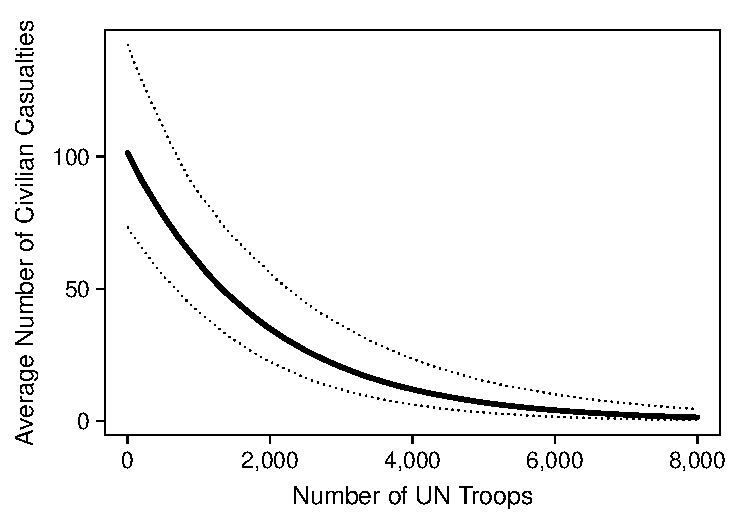
\includegraphics[scale = .8]{figs/hks-ev.pdf}
\caption{This figure shows expected number of civilian casualties as the number of U.N. troops increases.}\label{fig:hks-ci}
\end{center}
\end{figure}

% Direction
Noting that the relevant coefficients are statistically significant and correctly signed, Hultman, Kathman, and Shannon write:

\begin{quote}
The negative and statistically significant ($p < 0.001$) effects of \textit{UN Military Troops} and \textit{UN Police} suggest that as PKOs are increasingly supplied with soldiers and police forces, violence against civilians in civil war decreases (p. 9-10).
\end{quote}

% Magnitude
Hultman, Kathman, and Shannon argue that effect is not only statistically significant, but substantively important.

\begin{quote}
The figure shows that increasing the number of troops has a \emph{dramatic effect} on improving the safety of noncombatants. With no troops deployed to a conflict, the expected number of civilians killed in a given month is approximately 106. When the number of UN military troops increases to 8,000, the expected value of civilian deaths declines to 1.79. Conditional on the other variables being held at the specified values, supplying only several thousand military troops \emph{nearly mutes} violence completely as the number of troops approaches the upper values reported (p. 11, emphasis ours)
\end{quote}

\noindent They continue:

\begin{quote}
Bear in mind that the values presented are expected civilian deaths per month. These are \emph{not inconsequential} reductions in violence. Indeed, given that the average length of a conflict in these data is nearly 65 months, deploying highly equipped missions can \emph{mitigate or wholly avert humanitarian disasters} (p. 11, emphasis ours).
\end{quote}

% but they fail to take uncertainty into account
However, they do not explicitly take uncertainty into account when arguing for a meaningful effect. Instead, they only check that the \emph{estimate} is substantively important. They do not consider whether trivial effects are also plausible based on the data.

To assess whether their claim is robust to accounting for the uncertainty, we replicate their results and calculate first-differences and 90\% confidence intervals around the change in the expected civilian deaths as UN military troops increases. Figure \ref{fig:hks-ci} shows these confidence intervals. At an expense of roughly \$2 million, 2,000 troops leads to about 65 fewer civilian casualties, on average. However, the data suggest that the effect leads to \textit{at least} 45 fewer civilian casualties and possibly as many as 95. Similarly, an expense of about \$8 million, or 8,000 troops, leads to the prevention of approximately 100 civilian casualties. However, we can be confident that 8,000 troops prevents at least 70 civilian deaths and perhaps as many as 140. 

% summary of our point
In this case, the authors indeed have strong evidence for a \emph{dramatic effect}, even after uncertainty is taken into account. While the data support their claim, the authors can make a stronger argument for a meaningful effect, but explicitly accounting for uncertainty by substantively interpreting the range of plausible values rather than the point estimate.

\begin{figure}[H]
\begin{center}
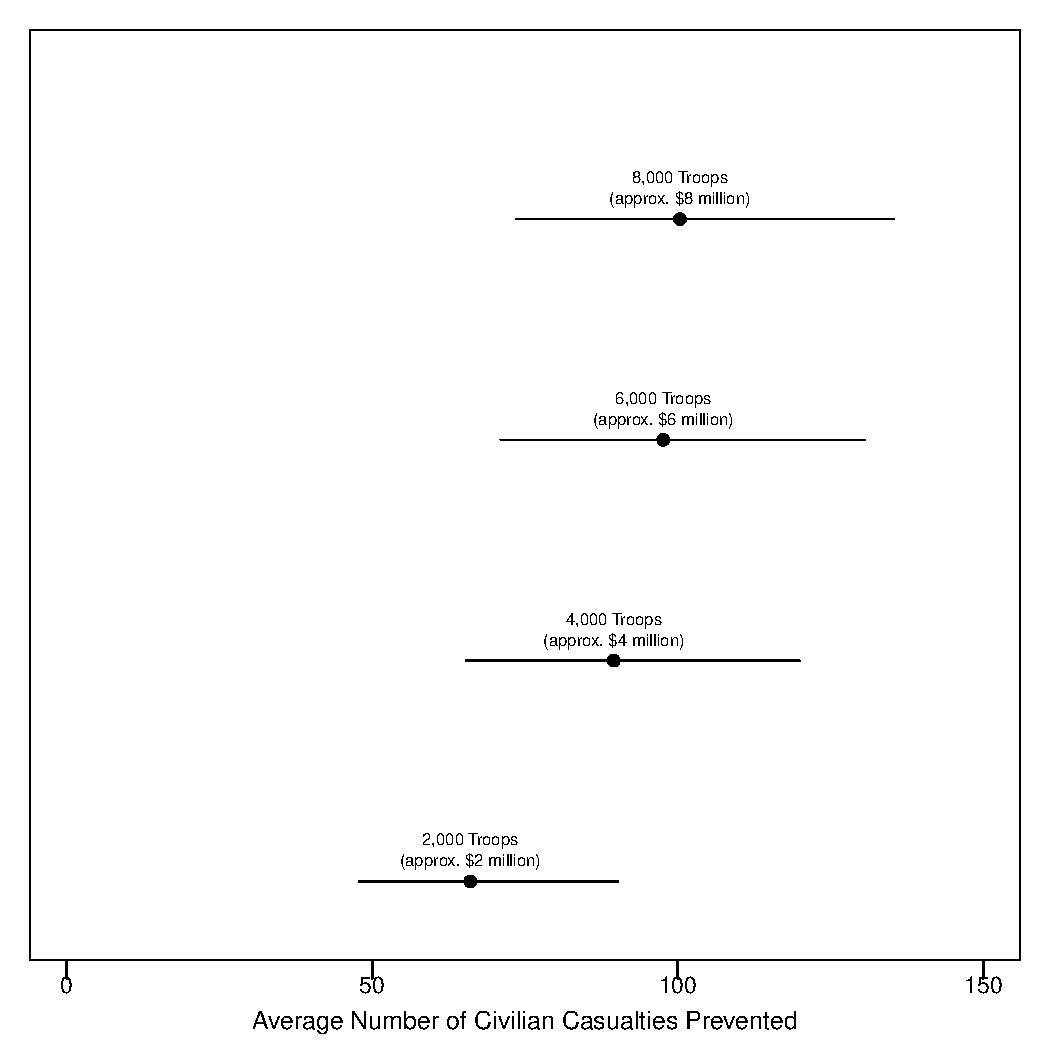
\includegraphics[scale = .8]{figs/hks-ci.pdf}
\caption{This figure provides first differences, in dollar and troop amounts, and their corresponding number of prevented civilian casualties.}\label{fig:hks-ci}
\end{center}
\end{figure}

\section*{Replication of Kam and Zechmeister (2013)}

% overview of kz
\cite{KamZechmeister2013} argue that name recognition increases a candidate's support directly, by increasing the candidate's approval, and indirectly, by informing voters about the candidate's viability. The authors present three lab experiments to demonstrate the causal link between their concepts of interest, but they use a field experiment to boost the external validity of the laboratory results. 

% the basic design
Through a clever design exploiting routes that parents must use to drop their kids off at school, Kam and Zechmeister expose half of parents in a particular geographic region to four yard signs displaying fictitious candidate Ben Griffin's name. The other half of parents are not exposed to any name and serve as a control group. The authors then survey the parents and ask them to indicate their top three choices for city council seats by choosing among five actual candidates and two fictional candidates (Ben Griffin, whose name appeared on yard signs and Milt Jenkins, whose name did not appear on any signs and who serves as a placebo). 

% the basic results
The authors summarize their results:

\begin{quote}
Did recognition spurred on by political yard signs increase support for Ben Griffin in the treatment group? To determine if this is so, we examine the extent to which survey respondents selected Ben Griffin as one of their top three choices for council. As shown in [their] Table 3, in the control condition, only 13.9\% of respondents placed Ben Griffin among their top three choices, but in the treatment condition, 23.9\% of respondents placed Ben Griffin among their top three choices. This 10 percentage point difference is sizable given the modesty of the treatment. In light of the small sample size, it is statistically significant at generous levels ($p \approx 0.13$, one-tailed).
\end{quote}

\noindent They continue:

\begin{quote}
we can examine the rates of selection of the two fictitious names, within each condition. Among the treated subjects, 23.9\% of subjects placed Ben Griffin in the top three set, but only 13.0\% placed Milt Jenkins in the top three set, a statistically significant difference at p < 0.09, one-tailed. Among the control subjects, 13.9\% placed Ben Griffin in the top three set, and the identical percentage, 13.9\%, placed Milt Jenkins in the top three set. The results from this field study lend generalizability to the claim established in our laboratory studies: name recognition increases candidate support in low- information elections.
\end{quote}

% are their claims robust to considering uncertainty?
But can we be confident that this effect is indeed ``sizable''? Are small effects plausible given the data? Figure \ref{fig:kz-ci} shows the estimated effects and 90\% confidence intervals. Notice that while the estimated effects are of borderline statistical significance, the estimated effects of about 10 percentage points are quite large. However, much smaller effects are plausible as well. Indeed, the authors cannot even reject the tiniest of effects with these data. While the estimated effects are ``large and significant,'' these data do not offer compelling evidence for a substantively meaningful effect.

\begin{figure}[H]
\begin{center}
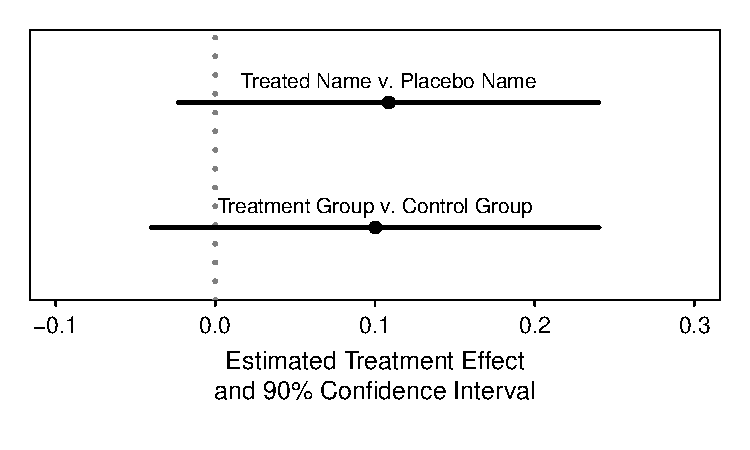
\includegraphics[scale = .8]{figs/kz-ci.pdf}
\caption{This figure provides the estimated treatment effect and 90\% confidence intervals for placing candidate roadsigns along a street which citizens regularly drive on the probability of ranking the named candidate in the top three of seven candidates. The top estimate compares the treatment with the control group (i.e., parents driving along different routes) and the bottom estimate compares the named candidate to the placebo candidate among parents driving along the route with the yard signs.}\label{fig:kz-ci}
\end{center}
\end{figure}

\section*{Discussion}

In this paper, we lay out an approach that allows researchers to make strong empirical arguments that effects of interest are substantively significant. However, we would like to suggest several caveats.

Our goal is not to bring past research into question or to suggest that researchers should never test a simple directional hypothesis. Instead, our goal is to provide future researchers with a tool to strengthen their claims and more clearly communicate their evidence to readers in many situations, though not all. Indeed, while testing a null hypothesis of exactly no effect has received ample criticism from methodologists (\citealt{Gill1999}, \citealt{Gross2014}, and \citealt{HillJones2014}), some researchers defend its merits (e.g., \citealt{Hagen1997} and \citealt{Wainer1999}). The method we propose, while powerful, has its own limitations.

In some situations, the scale or magnitude of the outcome or explanatory variable might not be interpretable, making the magnitude of effects difficult to discern. This can happen, for example, in observational studies in which the outcome or explanatory variables are measured poorly or in lab experiments, in which the experimental treatment might not map onto the real-world ``treatment.'' In this situations, a simple sign-and-significance approach is a compelling alternative.

\subsection*{Measurement Error}

% Measurement Error in the Outcome

In the special case of the normal-linear model, measurement error in the outcome variable in regression models simply increases the standard errors of the estimate and does not lead to bias (i.e., the error term simply becomes $e_i + u_i$, where $e_i$ is the usual residual and $u_i$ is the measurement error for observation $i$). However, this specific finding does not generalize to other models. Consider a logit model for example. Suppose that certain events are randomly misclassified. This has the effect of shifting the probability of an event toward one-half because the more outcome is more likely to be misclassified. As the probability of an event moves toward one-half, the marginal effects of all explanatory variables decrease. Thus, researchers must carefully consider the impact of measurement error in the outcome variable when making arguments about the magnitude of an effect.  

% Measurement Error in the Explanatory Variables

Some researchers claim that measurement errors in explanatory variables attenuate estimated effects by biasing the estimates toward zero. This would work against against researchers arguing for directional or substantively meaningful effects and lead to a conservative test. However, measurement errors in explanatory variables lead to attenuation only when the measurement error is random and uncorrelated with measurement error in the other explanatory variables. If measurement error exists in multiple variables and the errors are correlated, then the size and direction of the bias is quite difficult to discern. Researchers must carefully consider the impact of measurement error in the explanatory variables when making arguments about the magnitude of an effect.

% Summary paragraph of solutions

What, then, should be done about measurement error? The first step is to carefully choose the best measures of the key theoretical concepts. The second step is to identify any potential measurement error. If measurement error is present and cannot easily be corrected, then the researcher should carefully discuss the biases that will likely results from these errors. In some cases, the bias might strengthen the claim, and in other cases, the bias might weaken the claim. The important point is to carefully consider the potential bias.

\subsection*{Lab Experiments}

% Lab experiments

Lab experiments present a difficult environment for those arguing about the magnitude of an effect (as opposed to the direction). While some scholars, such as \cite{Gerber2011}, seem skeptical about the ability of lab experiments to determine the magnitude of an effect, \cite{JeritBarabasClifford2013} present evidence suggesting that lab experiments produces \textit{larger} effects than similar field experiments. They suggest that the larger effects occur due to (1) forced exposure to the treatment \citep{GainesKuklinski2011}, (2) the pristine lab environment \citep{Kinder2007}, (3) the obtrusiveness of the experiment (Webb et al. 2000), and (4) the time distance between the treatment and the outcome. These can combine to produce a smaller or larger effects in the lab, but Jerit, Barabas, and Clifford suggest that the effect should be larger on average.

In the case of lab experiments, the researcher should think careful about how the study design maps onto the key real-world concepts. For example, is their reason that a negative add shown in the laboratory has an effect similar in magnitude as an add viewed at home after dinner? It seems plausible that the effect occurs in the same \emph{direction}, but the \emph{magnitudes} might be quite different.

For example, \cite{MutzReeves2005}, in studying the effects of incivility on political trust, use treatments that represent quite extreme versions of the level of civility (extreme politeness and calm) and incivility (disrespect, eye-rolling, raising voices) that we might find in actual campaigns. There are good statistical reasons to rely on treatments with large effects--it increases the power of the study--but this strategy prevents the researcher from drawing meaningful inferences about the magnitude of the effect. Similarly, an experimenter asking a subject to read a newspaper article might have very different effects than the publication of the identical article outside of the lab environment.

This does not imply that lab experiments are overused or less important that other types of experiments. Indeed, the control that makes estimating magnitude of an effect difficult might make discovering the direction of an effect easier. The important point is to recognize that the ``effect'' in a lab experiment might correspond to the ``effect'' in the real world only in direction. Accordingly, researcher should carefully consider this possibility and, if necessary, adjust the empirical claims accordingly, focusing on direction and not magnitude, in this situation, the usual directional hypothesis test maps onto the substantive claim perfectly.


\subsection*{Conclusion}

In this paper, we have argued that researchers should explicitly test their substantive claims. In some cases this only requires testing a directional hypothesis. In other cases, this requires an explicit test for a meaningful effect. Our suggests suggestion that researchers formally test that effects lie above a threshold of substantive significance is not new (\citealt{Achen1982}, \citealt{Rainey2014}, and \citealt{Gross2014}; see also \citealt{EsareyDanneman2014}). However, explicit testing of substantive claims is not yet common practice and scholars rarely offer complete, substantive interpretations of the range of effects contain in confidence intervals. The current practice continues to be testing a directional research hypothesis and interpreting the substantive meaning of the estimate without taking into account the uncertainty surrounding the estimate. 

We hope that our discussion encourages researchers to move beyond the current practice. We hope that researchers begin to make precise claims about substantive significance and offer compelling evidence for those claims using explicit tests for meaningful effects or ``softly'' interpreting the range of values in the confidence interval. Using this approach, researchers will (1) compute quantities that are of direct substantive interest, (2) clarify claims about the effects they consider theoretically and/or normatively important, and (3) take the uncertainly of the estimates into account when assessing the evidence for their substantive claims. This leads more transparent substantive claims and clearer communication of the empirical evidence for these claims.

\singlespace 
\normalsize
\singlespace
\bibliographystyle{apsr_fs}
\bibliography{/Users/carlislerainey/Dropbox/papers/bibliography/bibliography.bib}

\end{document}